\section{Data Analysis} \label{data}
Three data is split into three main parts: \textit{demographics} (before playing the game), \textit{mid-questionnaire} (while playing the game) and \textit{post-questionnaire} (after playing the game). The mid-questionnaire consists of two parts. In the first part, participants describe the game feel in their own words. In the second part, participants rate the game feel on pre-defined words using Likert scales. The post-questionnaire is about game feel in general. The following analyzes the data from the three parts.

\subsection{Demographics}
As stated previously, the game was mainly shared on gaming websites. At the time of writing, 274 participants have played the game. Tables \ref{table:demographics1} and \ref{table:demographics2} show demographical data about the participants. Most of the participants rated themselves rather experienced with both playing videogames in general and playing 2D platforming games.

%%% This is how to insert a table %%%
\begin{table}[htbp]
\scriptsize
\centering
\begin{tabular}{|l|l|l|l|}
\hline
\textbf{Platform} & Windows Web: & Windows Exe: & Mac Web: \\
                  & 55,2\%      & 30,7\%      & 14,1\%  \\
\hline
\textbf{Gender}   & Male:        & Female:      & Other:   \\
                  & 93,6\%      & 5,7\%       & 0,7\%   \\
\hline
\textbf{Averages}      & Age:     & Framerate:            & Time spent:        \\
                  & 24,6 years  & 59,7 FPS           & 61 seconds/level        \\
\hline
\end{tabular}
\caption{Demographics data 1.}
\label{table:demographics1}
\end{table}

\begin{table}[h]
\scriptsize
\centering
\begin{tabular}{|l|ll|}
\hline
\textbf{Region}                      &                & \textbf{}               \\ \hline
\textit{Europe}                      & 70,6\%         &                         \\ \hline
\textit{Americas}                    & 26,7\%         &                         \\ \hline
\textit{Asia}                        & 1,9\%          &                         \\ \hline
\textit{Oceania}                     & 0\%            &                         \\ \hline
\textit{Africa}                      & 0,6\%          &                         \\ \hline
\textit{Other}                       & 0,2\%          &                         \\ \hline
\textit{\textbf{Experience with...}} & \textbf{Videogames} & \textbf{2D platformers} \\ \hline
\textit{1 (none)}                           & 0\%            & 0\%                     \\ \hline
\textit{2}                           & 0\%            & 3,1\%                   \\ \hline
\textit{3}                           & 0,6\%          & 10,1\%                  \\ \hline
\textit{4}                           & 4\%            & 14,1\%                  \\ \hline
\textit{5}                           & 9,6\%          & 23,2\%                  \\ \hline
\textit{6}                           & 22,5\%         & 16,9\%                  \\ \hline
\textit{7 (a lot)}                           & 63,3\%         & 32,6\%                  \\ \hline
\end{tabular}
\caption{Demographics data 2.}
\label{table:demographics2}
\end{table}

As stated in Section \ref{latinSection}, ideally there should be an equal amount of participants in each of the four Latin square sequences. However, as shown in Table \ref{table:latinSequenceNumber}, this is not the case. This might be due to either players quitting halfway, or that participants for some reason lost the Internet connection while trying to access the current Latin square number (in this case, the sequence was chosen randomly). Each time a participant collects three stars and answers the mid-questionnaire, data is logged. In total, 701 data logs were collected. Figure \ref{fig:retention} illustrates the retention rate of the participants.

%%% This is how to insert a table %%%
\begin{table}[htbp]
\scriptsize
\centering
\begin{tabular}{|c|c|}
\hline
 & \textbf{\# of participants}\\
 \hline
\textbf{Sequence 1} & 190\\
\hline
\textbf{Sequence 2} & 179\\
\hline
\textbf{Sequence 3} & 165\\
\hline
\textbf{Sequence 4} & 167\\
\hline
\end{tabular}
\caption{The number of participants in each of the four Latin square sequences.}
\label{table:latinSequenceNumber}
\end{table}

\begin{figure}[htbp]
\centering
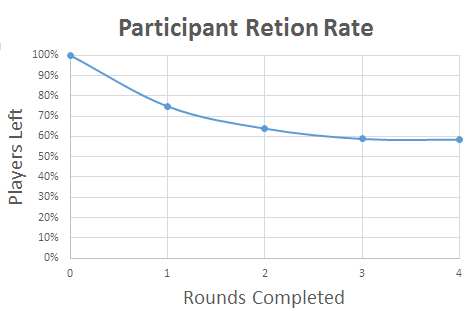
\includegraphics[width=0.4\textwidth]{Pics/retetionRate}
\caption{274 participants started the game, but not all completed the four rounds, presumably due to fatigue or boredom.}
\label{fig:retention}
\end{figure}

\subsection{Mid-questionnaire}
Whenever players collected three stars, they were met with a set of questions (see Figure \ref{fig:questionnaire}). In the first part, participants describe the game feel in their own words, while they in the second part rate pre-defined words on a 7-point Likert scale.

\subsubsection{Describing Game Feel in Own Words}
To get an overview of the words participants used, a word cloud has been generated (see Figure \ref{fig:wordcloud}). This illustrates the most commonly-used words, such as \textit{ball}, \textit{control}, \textit{fast}, \textit{heavy}, \textit{slow}, \textit{like}, \textit{responsive}, \textit{sluggish}, \textit{easy} and \textit{momentum}.

The words that the participants used to describe the game feel have manually, by a single person, been put into one or more of following nine categories (see Figure \ref{fig:coding1}). Note that a description can include words from multiple categories at once. The average word count for ground descriptions is 5,4 words.
\begin{itemize}[noitemsep,nolistsep]
\item Single words or multiple words?
\item Basic or complex words (basic words are root words that can stand on their own, e.g., \textit{heavy} and \textit{laggy}, whereas complex words consist of modifiers that somehow change the meaning of the root words, e.g., \textit{very fast} or \textit{a bit sluggish})?
\item Did the words describe a quality/opinion (using words such as \textit{fun}, \textit{too fast} or \textit{very annoying} or \textit{unrealistic})?
\item Did the words describe anything related to the difficulty; did the words use physical properties (\textit{like dragging through light mud}, using words such as \textit{force} and \textit{momentum})?
\item Did the words make comparisons to other games (\textit{like Mario} or \textit{like Mega Man})?
\item Did the words make comparisons to previous rounds of the game (\textit{similar to last round})?
\end{itemize}

\begin{figure}[htbp]
\centering
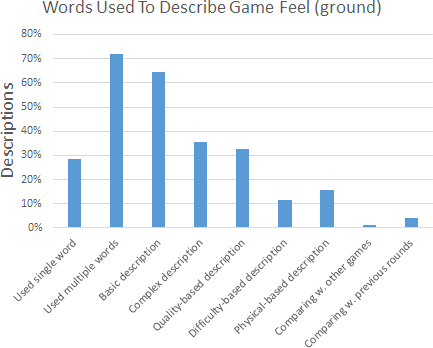
\includegraphics[width=\columnwidth]{Pics/coding1}
\caption{Coding1. NOTE: Coding not done yet.}
\label{fig:coding1}
\end{figure}

\begin{figure*}[htbp]
\centering
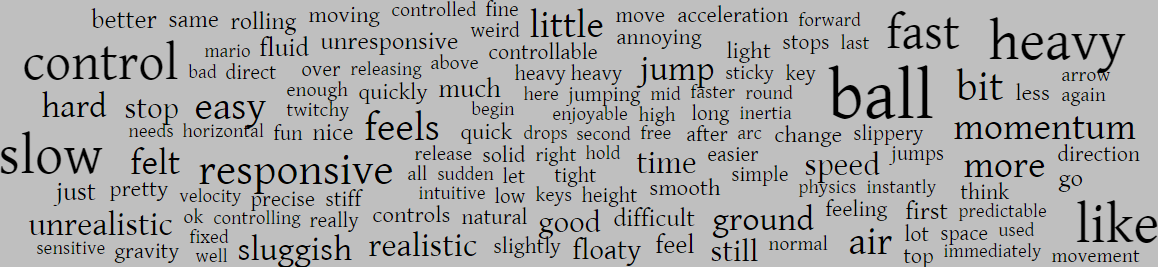
\includegraphics[width=1\textwidth]{Pics/wordcloud}
\caption{The 130 most commonly-used words to describe the feel of the controls (both on ground and in air). Bigger means a word has been used more frequently. Common words such as \textit{a}, \textit{also}, \textit{and}, \textit{have}, \textit{could}, etc. have been excluded. Created with WordItOut.com.}
\label{fig:wordcloud}
\end{figure*}

\subsubsection{Rating Game Feel with Pre-Defined Words}
Using a 7-point Likert scale, participants rated the game feel on the following pre-defined words.
\begin{itemize}[noitemsep,nolistsep]
\item Twitchy
\item Fluid
\item Stiff
\item Floaty
\item Responsive
\item Enjoyable
\item Difficult
\item How much they liked the controls
\item Frustration
\end{itemize}

%\begin{figure}[htbp]
%\centering
%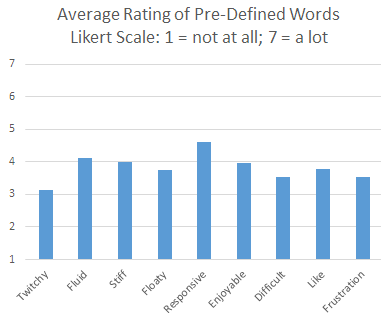
\includegraphics[width=0.35\textwidth]{Pics/average_rating}
%\caption{Averages of how participants rated the game feel across the pre-defined words.}
%\label{fig:average_rating}
%\end{figure}

One way to illustrate the responses is to plot the average ratings using acceleration and deceleration times, respectively (see Figures \ref{fig:acc_average_response} and \ref{fig:dec_average_response}). Even though one might be able to spot some slight tendencies, this way of showing the data is not accurate, since it splits up the acceleration and deceleration. The participants did not experience either in a vacuum; both were apparent all the time.

\begin{figure}[htbp]
\centering
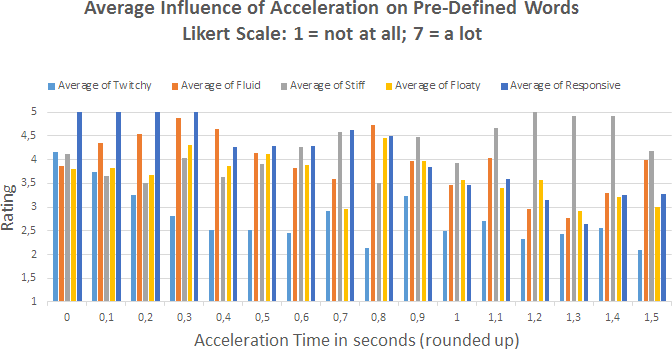
\includegraphics[width=0.97\columnwidth]{Pics/acc_average_response}
\caption{Average ratings with acceleration.}
\label{fig:acc_average_response}
\end{figure}

\begin{figure}[htbp]
\centering
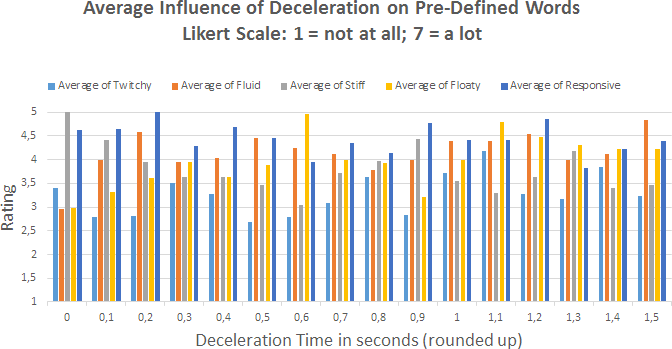
\includegraphics[width=0.97\columnwidth]{Pics/dec_average_response}
\caption{Average ratings with deceleration.}
\label{fig:dec_average_response}
\end{figure}

A different way to plot the data is to use both acceleration and deceleration at the same time. The following graphs show how the participants rated the game across the different words. For the case of clarity, only answers 1, 4 and 7 on the Likert scale are shown. Looking at the data, it appears as if the perceived contribution of the acceleration and deceleration times, respectively, aren't always equal.

When looking at Figure \ref{fig:twitchy}, it seems like the acceleration have a bigger influence than the deceleration when it comes to how \textit{twitchy} the game felt. Even with relatively high deceleration times (> 1 second), some participants still rated the game to feel very twitchy.

Figure \ref{fig:fluid} shows how \textit{fluid} participants perceived the game. Again, it is difficult to find a strong pattern, since participants with both small (< 0.4 seconds) and high (> 0.6 seconds) acceleration/deceleration times report the game to feel relatively fluid. However, it is clear that high acceleration time (> 0.6 seconds) results in a perception of low fluid.

With \textit{stiffness}, it appears that the deceleration has a greater influence than acceleration. This is evident in Figure \ref{fig:stiff}. Even with high acceleration times (> 0.6 seconds), participants still reported the game to fill stiff, as long as the deceleration time was below about 0.4 seconds.

Figure \ref{fig:floaty} shows a slight tendency towards high deceleration times (> 1 second) for a more \textit{floaty} feel. That being said, many reported gave the rating 4 around deceleration time 0.2 seconds.

With \textit{responsiveness}, there is a clear tendency towards acceleration having a bigger influence than deceleration. It seems like acceleration times below 0.2 seconds makes the game feel responsive. Likewise, when it comes to \textit{frustration}, Figure \ref{fig:frustration} shows that acceleration and deceleration times above 0.2 seconds makes participant feel frustration.

%width=\columnwidth
\begin{figure*}[htbp]
\centering
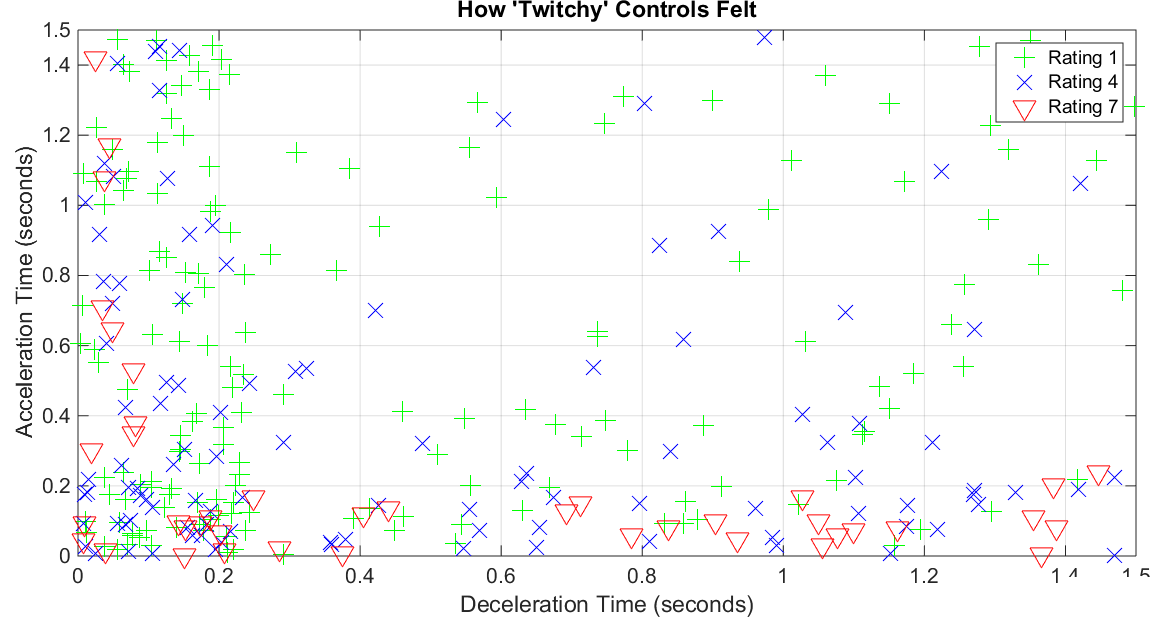
\includegraphics[width=0.67\textwidth]{Pics/Classes/Twitchy_classes}
\caption{Players' self-reported perception on how twitchy the controls felt, rated using a 7-point Likert scale (only 1, 4 and 7 are shown).}
\label{fig:twitchy}
\end{figure*}

\begin{figure*}[htbp]
\centering
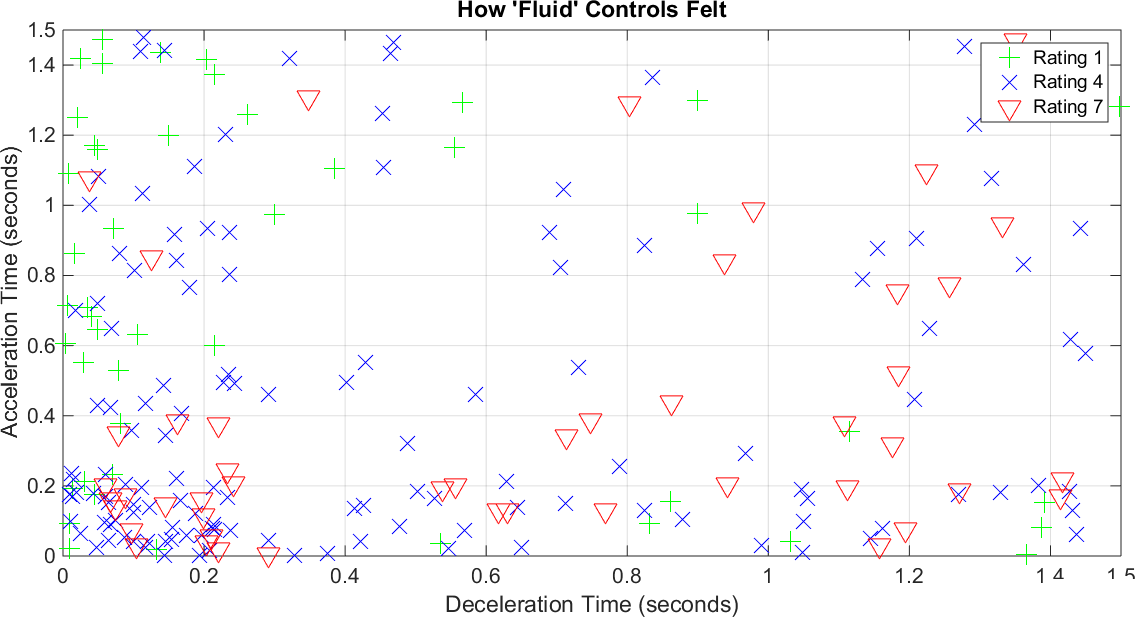
\includegraphics[width=0.67\textwidth]{Pics/Classes/Fluid_classes}
\caption{Players' self-reported perception on how fluid the controls felt, rated using a 7-point Likert scale (only 1, 4 and 7 are shown).}
\label{fig:fluid}
\end{figure*}

\begin{figure*}[htbp]
\centering
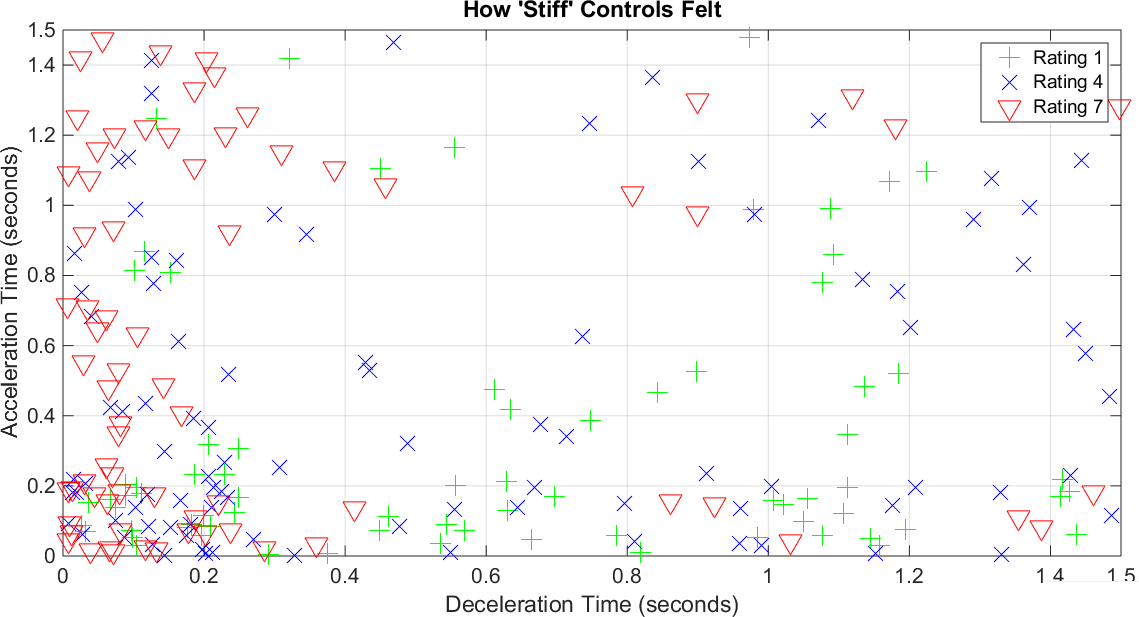
\includegraphics[width=0.67\textwidth]{Pics/Classes/Stiff_classes}
\caption{Players' self-reported perception on how stiff the controls felt, rated using a 7-point Likert scale (only 1, 4 and 7 are shown).}
\label{fig:stiff}
\end{figure*}

\begin{figure*}[htbp]
\centering
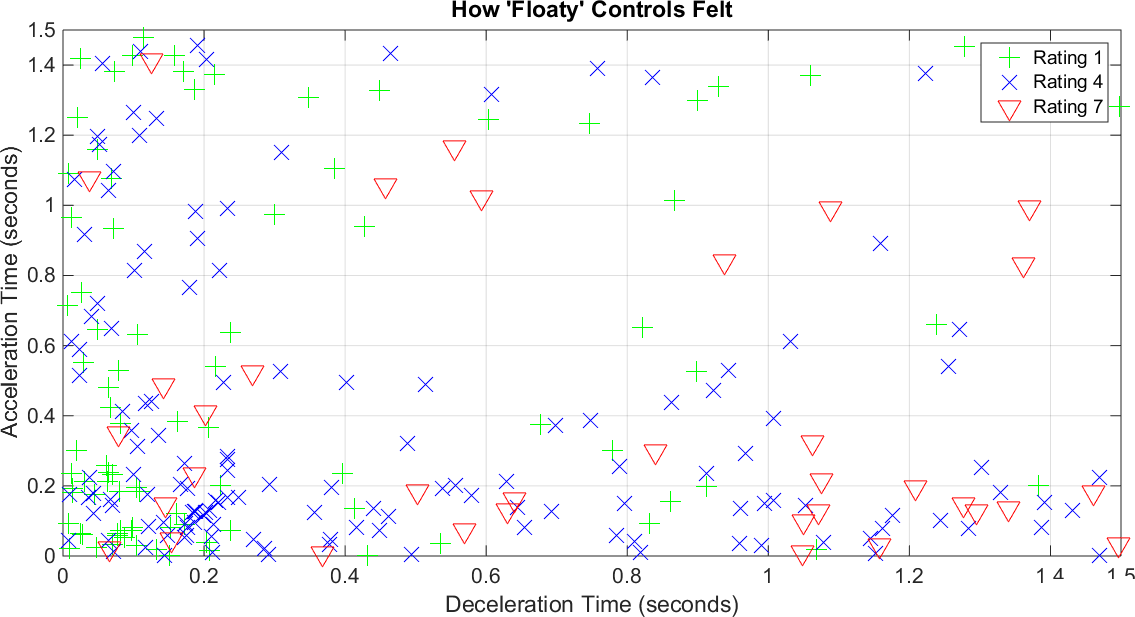
\includegraphics[width=0.67\textwidth]{Pics/Classes/Floaty_classes}
\caption{Players' self-reported perception on how floaty the controls felt, rated using a 7-point Likert scale (only 1, 4 and 7 are shown).}
\label{fig:floaty}
\end{figure*}

\begin{figure*}[htbp]
\centering
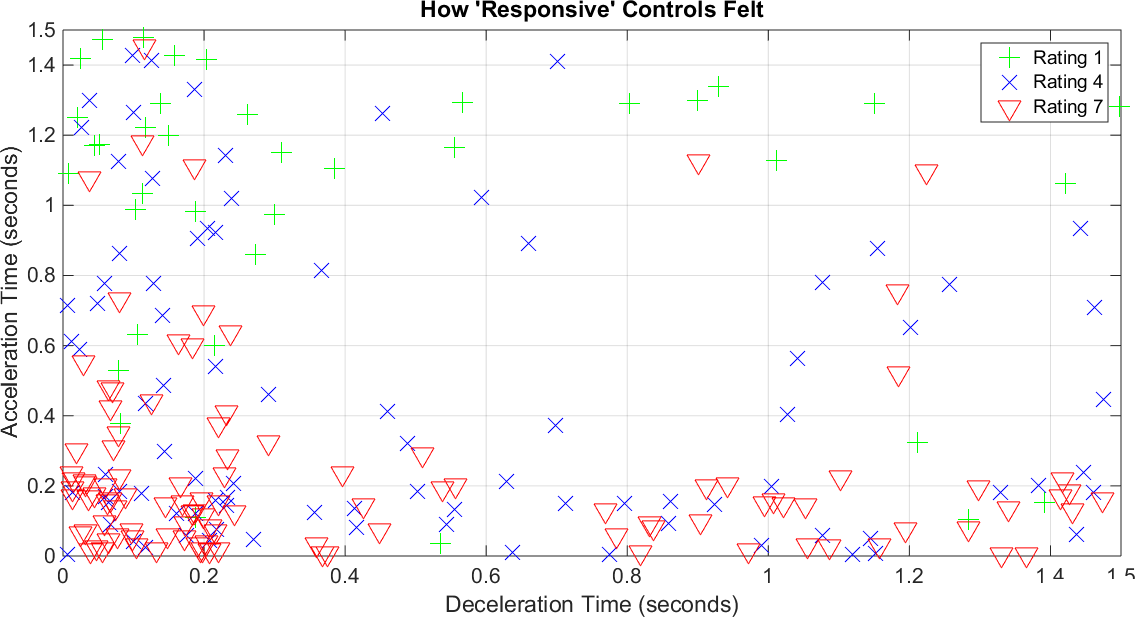
\includegraphics[width=0.67\textwidth]{Pics/Classes/Responsive_classes}
\caption{Players' self-reported perception on how responsive the controls felt, rated using a 7-point Likert scale (only 1, 4 and 7 are shown).}
\label{fig:responsive}
\end{figure*}

\begin{figure*}[htbp]
\centering
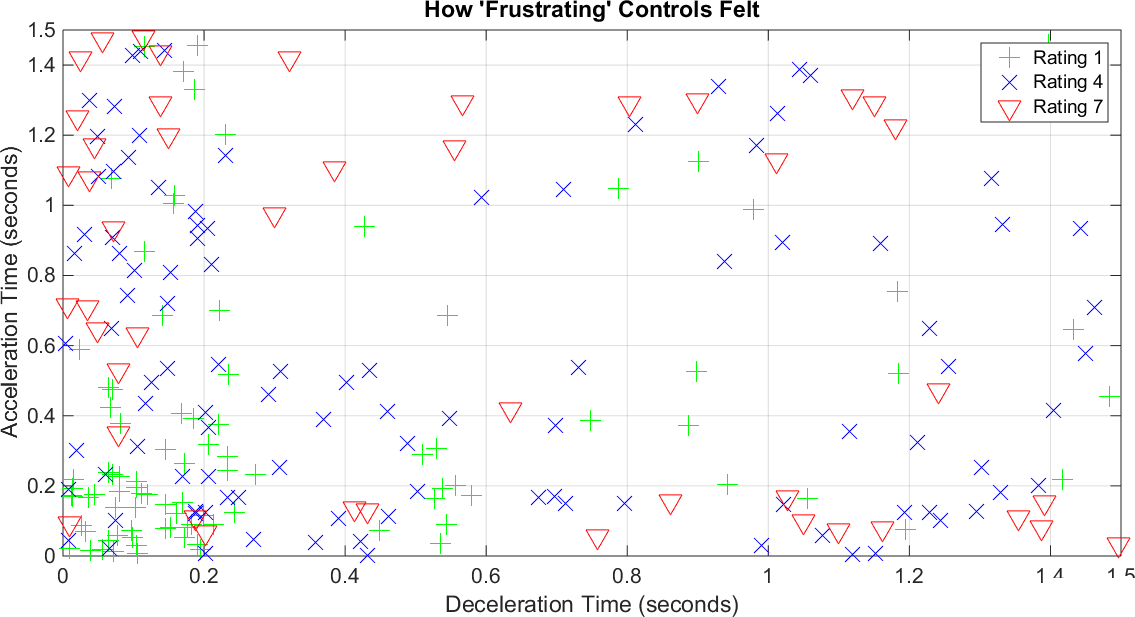
\includegraphics[width=0.67\textwidth]{Pics/Classes/Frustration_classes}
\caption{Players' self-reported perception on how frustrating the controls felt, rated using a 7-point Likert scale (only 1, 4 and 7 are shown).}
\label{fig:frustration}
\end{figure*}

A different way to visualize the data is to take the averages of the acceleration/deceleration times for each of the ratings, e.g., what are the average acceleration/deceleration times for twitchy rating 1, rating 2, rating 3, etc. However, since a Likert scale consists of ordinal values, there is no guarantee that a rating difference of e.g. 1 represents an equal conceptual change, since the scale might be used differently by different participants. For instance, some participants might be hesitant to use the extreme values 1 (not at all) and 7 (a lot), while others might spread their answers across the whole scale \cite{cunningham}. Because of this, in the following graphs, the averages have been put into three weighted categories, so that the extreme ends contribute more. The \textit{low rating} curve consists of ratings 1 (70\%), 2 (20\%) and 3 (10\%). The \textit{mid rating} curve consists of ratings 3 (25\%), 4 (50\%) and 5 (25\%). The \textit{high rating} consists of ratings 5 (10\%), 6 (20\%) and 7 (70\%). Using these numbers, it is now possible to draw attack/deceleration curves (see Figures \ref{fig:curve_twitchy}, \ref{fig:curve_fluid}, \ref{fig:curve_stiff}, \ref{fig:curve_floaty} and \ref{fig:curve_floaty}). For all curves, the sustain time is 1 second. The numbers in square brackets represent acceleration and deceleration times.

At first glance, most of the curves seem similar. However, when comparing the three curves from the same word, there are some differences. For instance, there is a difference of about 360 milliseconds between the deceleration time in \textit{low rating} and \textit{high rating} in the \textit{floaty}. curve. Also, it should be noted that the difference words are not mutually exclusive, i.e., the controls can feel floaty and fluid at the same time.

\begin{figure}[htbp]
\centering
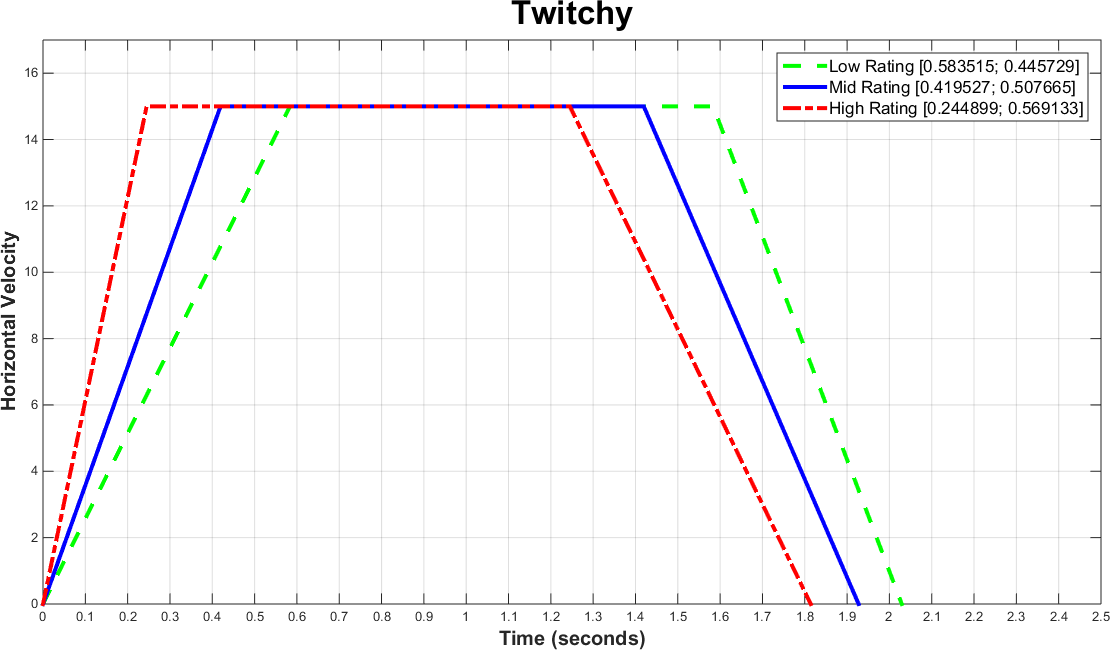
\includegraphics[width=0.9\columnwidth]{Pics/Curves/Twitchy_curve}
\caption{Average curves of twitchy controls.}
\label{fig:curve_twitchy}
\end{figure}

\begin{figure}[htbp]
\centering
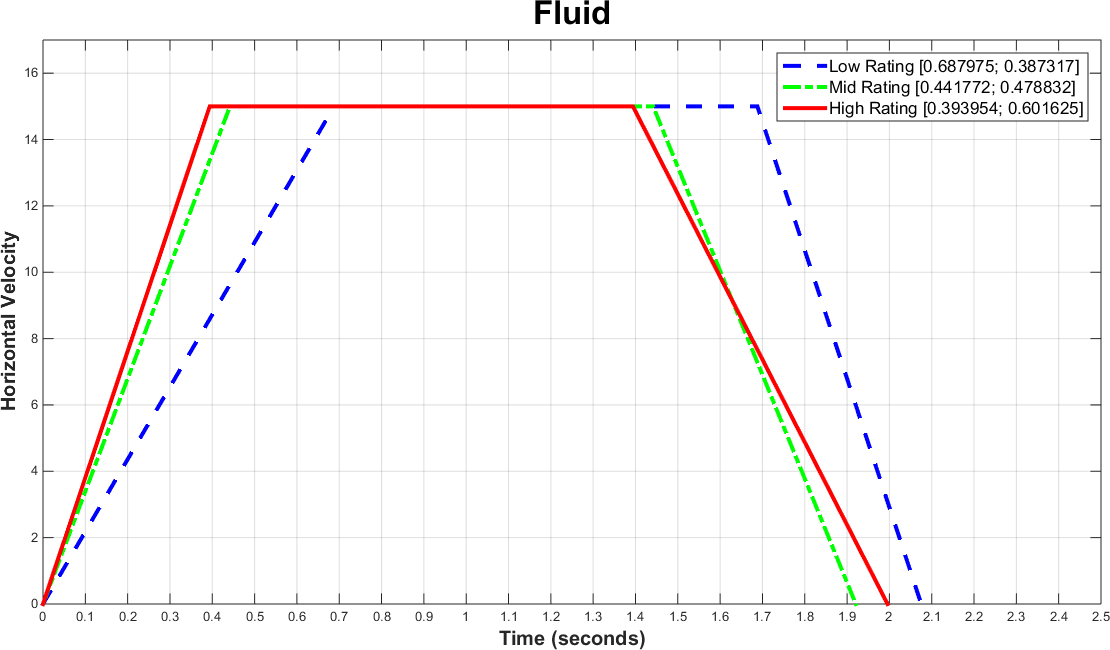
\includegraphics[width=0.9\columnwidth]{Pics/Curves/Fluid_curve}
\caption{Average curves of fluid controls.}
\label{fig:curve_fluid}
\end{figure}

\begin{figure}[htbp]
\centering
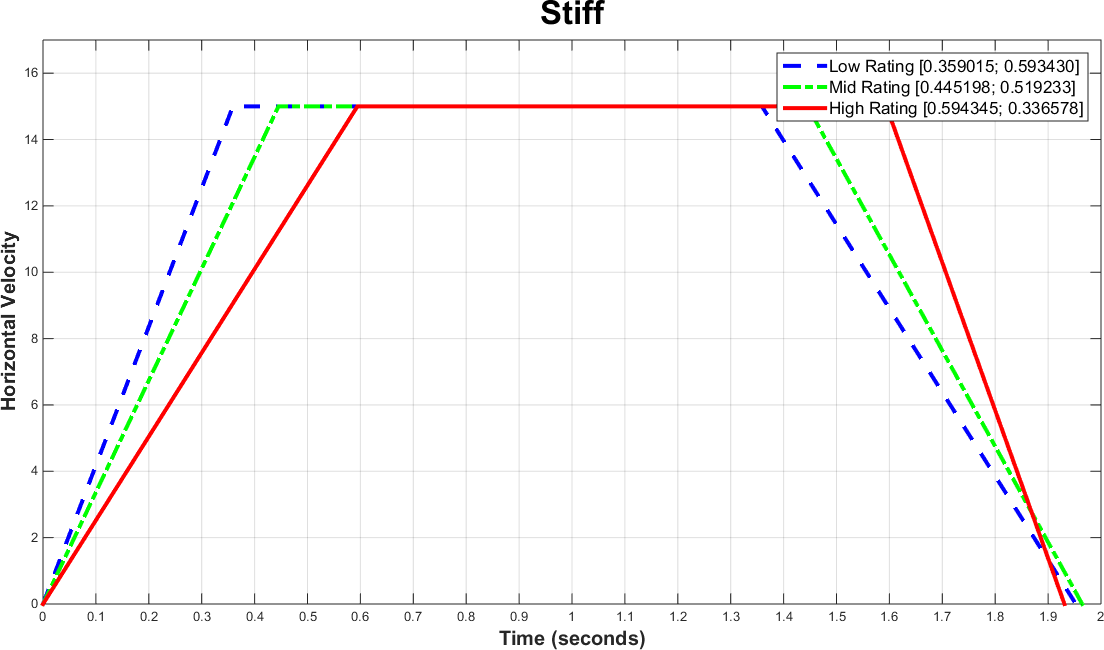
\includegraphics[width=0.9\columnwidth]{Pics/Curves/Stiff_curve}
\caption{Average curves of stiff controls.}
\label{fig:curve_stiff}
\end{figure}

\begin{figure}[htbp]
\centering
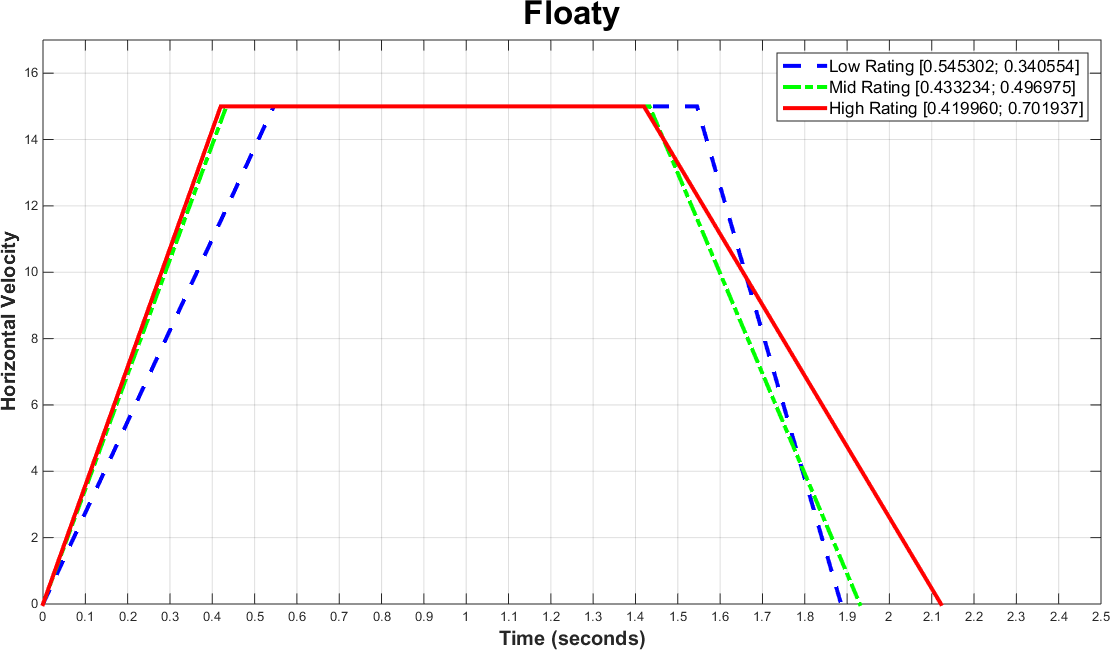
\includegraphics[width=0.9\columnwidth]{Pics/Curves/Floaty_curve}
\caption{Average curves of floaty controls.}
\label{fig:curve_floaty}
\end{figure}

\begin{figure}[htbp]
\centering
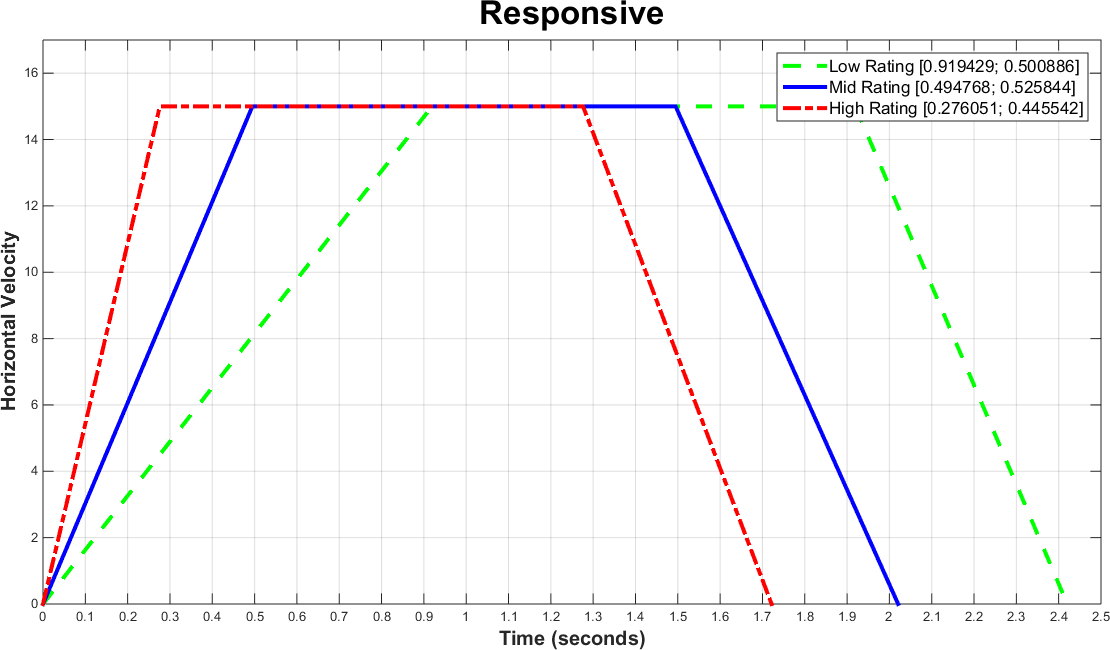
\includegraphics[width=0.9\columnwidth]{Pics/Curves/Responsive_curve}
\caption{Average curves of responsive controls.}
\label{fig:curve_responsive}
\end{figure}

\subsection{Post-questionnaire}
When completing the fourth round of the game, a link was shown to a Google Forms questionnaire. At the time of writing, 146 participants have taken part in this post-questionnaire.